 \documentclass[11pt,addpoints,answers]{exam}
%-----------------------------------------------------------------------------
% PACKAGES AND OTHER DOCUMENT CONFIGURATIONS
%-----------------------------------------------------------------------------

\usepackage[margin=1in]{geometry}
\usepackage{amsmath, amsfonts}
\usepackage{enumerate}
\usepackage{graphicx}
\usepackage{titling}
\usepackage{url}
\usepackage{xfrac}
\usepackage{natbib}
\usepackage{amssymb}
\usepackage{amsthm}
\usepackage{paralist}
\usepackage{epstopdf}
\usepackage{tabularx}
\usepackage{longtable}
\usepackage{multirow}
\usepackage{multicol}
\usepackage[colorlinks=true,urlcolor=blue]{hyperref}
\usepackage{algorithm}
\usepackage{algorithmicx}
\usepackage[noend]{algpseudocode}
\usepackage{float}
\usepackage{enumerate}
\usepackage{array}
\usepackage{environ}
\usepackage{times}
\usepackage{textcomp}
\usepackage{caption}
\usepackage{parskip} % For NIPS style paragraphs.
\usepackage[compact]{titlesec} % Less whitespace around titles
\usepackage[inline]{enumitem} % For inline enumerate* and itemize*
\usepackage{datetime}
\usepackage{comment}
% \usepackage{minted}
\usepackage{lastpage}
\usepackage{color}
% \usepackage{xcolor}
\usepackage[dvipsnames]{xcolor}
\usepackage[final]{listings}
\usepackage{tikz}
\usetikzlibrary{shapes,decorations}
\usepackage{framed}
\usepackage{booktabs}
\usepackage{cprotect}
\usepackage{verbatimbox}
\usepackage{multicol}
\usepackage{hyperref}
\usepackage{subcaption}
\usepackage{mathtools} % For drcases
\usepackage{cancel}
\usepackage[many]{tcolorbox}
\usepackage{soul}
\usepackage[bottom]{footmisc}
\usepackage{bm}
\usepackage{wasysym}
\usepackage{bbm}

\usepackage{tikz}
\usetikzlibrary{arrows}
\usetikzlibrary{arrows.meta}
\usetikzlibrary{shapes.geometric}
\usetikzlibrary{positioning, arrows, automata, calc}

\newtcolorbox[]{your_solution}[1][]{%
    % breakable,
    enhanced,
    nobeforeafter,
    colback=white,
    title=Your Answer,
    sidebyside align=top,
    box align=top,
    #1
}

%%%%%%%%%%%%%%%%%%%%%%%%%%%%%%%%%%%%%%%%%%%
% Formatting for \CorrectChoice of "exam" %
%%%%%%%%%%%%%%%%%%%%%%%%%%%%%%%%%%%%%%%%%%%

\CorrectChoiceEmphasis{}
\checkedchar{\blackcircle}

%%%%%%%%%%%%%%%%%%%%%%%%%%%%%%%%%%%%%%%%%%%
% Better numbering                        %
%%%%%%%%%%%%%%%%%%%%%%%%%%%%%%%%%%%%%%%%%%%

% \numberwithin{equation}{section} % Number equations within sections (i.e. 1.1, 1.2, 2.1, 2.2 instead of 1, 2, 3, 4)
% \numberwithin{figure}{section} % Number figures within sections (i.e. 1.1, 1.2, 2.1, 2.2 instead of 1, 2, 3, 4)
% \numberwithin{table}{section} % Number tables within sections (i.e. 1.1, 1.2, 2.1, 2.2 instead of 1, 2, 3, 4)

%%%%%%%%%%%%%%%%%%%%%%%%%%%%%%%%%%%%%%%%%%
% Custom commands                        %
%%%%%%%%%%%%%%%%%%%%%%%%%%%%%%%%%%%%%%%%%%
\newcommand{\blackcircle}{\tikz\draw[black,fill=black] (0,0) circle (1ex);}
\renewcommand{\circle}{\tikz\draw[black] (0,0) circle (1ex);}
\newcommand{\vc}[1]{\boldsymbol{#1}}
\newcommand{\adj}[1]{\frac{\partial \ell}{\partial #1}}
\newcommand{\chain}[2]{\adj{#2} = \adj{#1}\frac{\partial #1}{\partial #2}}
\newcommand{\ntset}{test}

% mathcal
\newcommand{\Ac}{\mathcal{A}}
\newcommand{\Bc}{\mathcal{B}}
\newcommand{\Cc}{\mathcal{C}}
\newcommand{\Dc}{\mathcal{D}}
\newcommand{\Ec}{\mathcal{E}}
\newcommand{\Fc}{\mathcal{F}}
\newcommand{\Gc}{\mathcal{G}}
\newcommand{\Hc}{\mathcal{H}}
\newcommand{\Ic}{\mathcal{I}}
\newcommand{\Jc}{\mathcal{J}}
\newcommand{\Kc}{\mathcal{K}}
\newcommand{\Lc}{\mathcal{L}}
\newcommand{\Mc}{\mathcal{M}}
\newcommand{\Nc}{\mathcal{N}}
\newcommand{\Oc}{\mathcal{O}}
\newcommand{\Pc}{\mathcal{P}}
\newcommand{\Qc}{\mathcal{Q}}
\newcommand{\Rc}{\mathcal{R}}
\newcommand{\Sc}{\mathcal{S}}
\newcommand{\Tc}{\mathcal{T}}
\newcommand{\Uc}{\mathcal{U}}
\newcommand{\Vc}{\mathcal{V}}
\newcommand{\Wc}{\mathcal{W}}
\newcommand{\Xc}{\mathcal{X}}
\newcommand{\Yc}{\mathcal{Y}}
\newcommand{\Zc}{\mathcal{Z}}

% mathbb
\newcommand{\Ab}{\mathbb{A}}
\newcommand{\Bb}{\mathbb{B}}
\newcommand{\Cb}{\mathbb{C}}
\newcommand{\Db}{\mathbb{D}}
\newcommand{\Eb}{\mathbb{E}}
\newcommand{\Fb}{\mathbb{F}}
\newcommand{\Gb}{\mathbb{G}}
\newcommand{\Hb}{\mathbb{H}}
\newcommand{\Ib}{\mathbb{I}}
\newcommand{\Jb}{\mathbb{J}}
\newcommand{\Kb}{\mathbb{K}}
\newcommand{\Lb}{\mathbb{L}}
\newcommand{\Mb}{\mathbb{M}}
\newcommand{\Nb}{\mathbb{N}}
\newcommand{\Ob}{\mathbb{O}}
\newcommand{\Pb}{\mathbb{P}}
\newcommand{\Qb}{\mathbb{Q}}
\newcommand{\Rb}{\mathbb{R}}
\newcommand{\Sb}{\mathbb{S}}
\newcommand{\Tb}{\mathbb{T}}
\newcommand{\Ub}{\mathbb{U}}
\newcommand{\Vb}{\mathbb{V}}
\newcommand{\Wb}{\mathbb{W}}
\newcommand{\Xb}{\mathbb{X}}
\newcommand{\Yb}{\mathbb{Y}}
\newcommand{\Zb}{\mathbb{Z}}

% mathbf lowercase
\newcommand{\av}{\mathbf{a}}
\newcommand{\bv}{\mathbf{b}}
\newcommand{\cv}{\mathbf{c}}
\newcommand{\dv}{\mathbf{d}}
\newcommand{\ev}{\mathbf{e}}
\newcommand{\fv}{\mathbf{f}}
\newcommand{\gv}{\mathbf{g}}
\newcommand{\hv}{\mathbf{h}}
\newcommand{\iv}{\mathbf{i}}
\newcommand{\jv}{\mathbf{j}}
\newcommand{\kv}{\mathbf{k}}
\newcommand{\lv}{\mathbf{l}}
\newcommand{\mv}{\mathbf{m}}
\newcommand{\nv}{\mathbf{n}}
\newcommand{\ov}{\mathbf{o}}
\newcommand{\pv}{\mathbf{p}}
\newcommand{\qv}{\mathbf{q}}
\newcommand{\rv}{\mathbf{r}}
\newcommand{\sv}{\mathbf{s}}
\newcommand{\tv}{\mathbf{t}}
\newcommand{\uv}{\mathbf{u}}
\newcommand{\vv}{\mathbf{v}}
\newcommand{\wv}{\mathbf{w}}
\newcommand{\xv}{\mathbf{x}}
\newcommand{\yv}{\mathbf{y}}
\newcommand{\zv}{\mathbf{z}}

% mathbf uppercase
\newcommand{\Av}{\mathbf{A}}
\newcommand{\Bv}{\mathbf{B}}
\newcommand{\Cv}{\mathbf{C}}
\newcommand{\Dv}{\mathbf{D}}
\newcommand{\Ev}{\mathbf{E}}
\newcommand{\Fv}{\mathbf{F}}
\newcommand{\Gv}{\mathbf{G}}
\newcommand{\Hv}{\mathbf{H}}
\newcommand{\Iv}{\mathbf{I}}
\newcommand{\Jv}{\mathbf{J}}
\newcommand{\Kv}{\mathbf{K}}
\newcommand{\Lv}{\mathbf{L}}
\newcommand{\Mv}{\mathbf{M}}
\newcommand{\Nv}{\mathbf{N}}
\newcommand{\Ov}{\mathbf{O}}
\newcommand{\Pv}{\mathbf{P}}
\newcommand{\Qv}{\mathbf{Q}}
\newcommand{\Rv}{\mathbf{R}}
\newcommand{\Sv}{\mathbf{S}}
\newcommand{\Tv}{\mathbf{T}}
\newcommand{\Uv}{\mathbf{U}}
\newcommand{\Vv}{\mathbf{V}}
\newcommand{\Wv}{\mathbf{W}}
\newcommand{\Xv}{\mathbf{X}}
\newcommand{\Yv}{\mathbf{Y}}
\newcommand{\Zv}{\mathbf{Z}}

% bold greek lowercase
\newcommand{\alphav     }{\boldsymbol \alpha     }
\newcommand{\betav      }{\boldsymbol \beta      }
\newcommand{\gammav     }{\boldsymbol \gamma     }
\newcommand{\deltav     }{\boldsymbol \delta     }
\newcommand{\epsilonv   }{\boldsymbol \epsilon   }
\newcommand{\varepsilonv}{\boldsymbol \varepsilon}
\newcommand{\zetav      }{\boldsymbol \zeta      }
\newcommand{\etav       }{\boldsymbol \eta       }
\newcommand{\thetav     }{\boldsymbol \theta     }
\newcommand{\varthetav  }{\boldsymbol \vartheta  }
\newcommand{\iotav      }{\boldsymbol \iota      }
\newcommand{\kappav     }{\boldsymbol \kappa     }
\newcommand{\varkappav  }{\boldsymbol \varkappa  }
\newcommand{\lambdav    }{\boldsymbol \lambda    }
\newcommand{\muv        }{\boldsymbol \mu        }
\newcommand{\nuv        }{\boldsymbol \nu        }
\newcommand{\xiv        }{\boldsymbol \xi        }
\newcommand{\omicronv   }{\boldsymbol \omicron   }
\newcommand{\piv        }{\boldsymbol \pi        }
\newcommand{\varpiv     }{\boldsymbol \varpi     }
\newcommand{\rhov       }{\boldsymbol \rho       }
\newcommand{\varrhov    }{\boldsymbol \varrho    }
\newcommand{\sigmav     }{\boldsymbol \sigma     }
\newcommand{\varsigmav  }{\boldsymbol \varsigma  }
\newcommand{\tauv       }{\boldsymbol \tau       }
\newcommand{\upsilonv   }{\boldsymbol \upsilon   }
\newcommand{\phiv       }{\boldsymbol \phi       }
\newcommand{\varphiv    }{\boldsymbol \varphi    }
\newcommand{\chiv       }{\boldsymbol \chi       }
\newcommand{\psiv       }{\boldsymbol \psi       }
\newcommand{\omegav     }{\boldsymbol \omega     }

% bold greek uppercase
\newcommand{\Gammav     }{\boldsymbol \Gamma     }
\newcommand{\Deltav     }{\boldsymbol \Delta     }
\newcommand{\Thetav     }{\boldsymbol \Theta     }
\newcommand{\Lambdav    }{\boldsymbol \Lambda    }
\newcommand{\Xiv        }{\boldsymbol \Xi        }
\newcommand{\Piv        }{\boldsymbol \Pi        }
\newcommand{\Sigmav     }{\boldsymbol \Sigma     }
\newcommand{\Upsilonv   }{\boldsymbol \Upsilon   }
\newcommand{\Phiv       }{\boldsymbol \Phi       }
\newcommand{\Psiv       }{\boldsymbol \Psi       }
\newcommand{\Omegav     }{\boldsymbol \Omega     }

%%%%%%%%%%%%%%%%%%%%%%%%%%%%%%%%%%%%%%%%%%%
% Code highlighting with listings         %
%%%%%%%%%%%%%%%%%%%%%%%%%%%%%%%%%%%%%%%%%%%

\definecolor{bluekeywords}{rgb}{0.13,0.13,1}
\definecolor{greencomments}{rgb}{0,0.5,0}
\definecolor{redstrings}{rgb}{0.9,0,0}
\definecolor{light-gray}{gray}{0.95}

\newcommand{\MYhref}[3][blue]{\href{#2}{\color{#1}{#3}}}%

\definecolor{dkgreen}{rgb}{0,0.6,0}
\definecolor{gray}{rgb}{0.5,0.5,0.5}
\definecolor{mauve}{rgb}{0.58,0,0.82}

\lstdefinelanguage{Shell}{
  keywords={tar, cd, make},
  %keywordstyle=\color{bluekeywords}\bfseries,
  alsoletter={+},
  ndkeywords={python3, python, py, javac, java, gcc, c, g++, cpp, .txt, octave, m, .tar},
  %ndkeywordstyle=\color{bluekeywords}\bfseries,
  identifierstyle=\color{black},
  sensitive=false,
  comment=[l]{//},
  morecomment=[s]{/*}{*/},
  commentstyle=\color{purple}\ttfamily,
  %stringstyle=\color{red}\ttfamily,
  morestring=[b]',
  morestring=[b]",
  backgroundcolor = \color{light-gray}
}

\lstset{columns=fixed, basicstyle=\ttfamily,
    backgroundcolor=\color{light-gray},xleftmargin=0.5cm,frame=tlbr,framesep=4pt,framerule=0pt}

\newcommand{\emptysquare}{{\LARGE $\square$}\ \ }
\newcommand{\filledsquare}{{\LARGE $\boxtimes$}\ \ }
\def \ifempty#1{\def\temp{#1} \ifx\temp\empty }


% \newcommand{\squaresolutionspace}[2][\emptysquare]{\newline #1}{#2}
\def \squaresolutionspace#1{ \ifempty{#1} \emptysquare \else #1\hspace{0.75pt}\fi}


\newcommand{\emptycircle}{{\LARGE $\fullmoon$}\ \ }
\newcommand{\filledcircle}{{\LARGE $\newmoon$}\ \ }
\def \circlesolutionspace#1{ \ifempty{#1} \emptycircle \else #1\hspace{0.75pt}\fi}
%%%%%%%%%%%%%%%%%%%%%%%%%%%%%%%%%%%%%%%%%%%
% Custom box for highlights               %
%%%%%%%%%%%%%%%%%%%%%%%%%%%%%%%%%%%%%%%%%%%

% Define box and box title style
\tikzstyle{mybox} = [fill=blue!10, very thick,
    rectangle, rounded corners, inner sep=1em, inner ysep=1em]

% \newcommand{\notebox}[1]{
% \begin{tikzpicture}
% \node [mybox] (box){%
%     \begin{minipage}{\textwidth}
%     #1
%     \end{minipage}
% };
% \end{tikzpicture}%
% }

\NewEnviron{notebox}{

\begin{tikzpicture}
\node [mybox] (box){
    \begin{minipage}{0.95\textwidth}
        \BODY
    \end{minipage}
};
\end{tikzpicture}
}

%%%%%%%%%%%%%%%%%%%%%%%%%%%%%%%%%%%%%%%%%%%
% Commands showing / hiding solutions     %
%%%%%%%%%%%%%%%%%%%%%%%%%%%%%%%%%%%%%%%%%%%
\newcommand{\solutionspace}[4]{\fbox{\begin{minipage}[t][#1][t]{#2} \textbf{#3} \solution{}{#4} \end{minipage}}}
%% To HIDE SOLUTIONS (to post at the website for students), set this value to 0: \def\issoln{0}
% \def\issoln{0}
\def\issoln{1}
% Some commands to allow solutions to be embedded in the assignment file.
\ifcsname issoln\endcsname \else \def\issoln{1} \fi
% Default to an empty solutions environ.
\NewEnviron{soln}{}{}
\if\issoln 1
% Otherwise, include solutions as below.
 \RenewEnviron{soln}{
    \leavevmode\color{red}\ignorespaces   %textbf{Solution} \BODY
    \BODY
 }{}
\fi

%% qauthor environment:
% Default to an empty qauthor environ.
\NewEnviron{qauthor}{}{}

%% To HIDE TAGS set this value to 0:
\def\showtags{0}
%%%%%%%%%%%%%%%%
\ifcsname showtags\endcsname \else \def\showtags{1} \fi
% Default to an empty tags environ.
\NewEnviron{tags}{}{}
\if\showtags 1
% Otherwise, include solutions as below.
\RenewEnviron{tags}{
    \fbox{
    \leavevmode\color{blue}\ignorespaces
    \textbf{TAGS:} \texttt{\url{\BODY}}
    }
    \vspace{-.5em}
}{}
\fi

% Default to an empty learning objective environment
\NewEnviron{qlearningobjective}{}

%%%%%%%%%%%%%%%%%%%%%%%%%%%%%%%%%%%%%%%%%%%
% Commands for customizing the assignment %
%%%%%%%%%%%%%%%%%%%%%%%%%%%%%%%%%%%%%%%%%%%

\newcommand{\courseNum}{10-301 / 10-601}
\newcommand{\courseName}{Introduction to Machine Learning}
\newcommand{\courseSem}{Spring 2024}
\newcommand{\courseUrl}{\url{http://www.cs.cmu.edu/~mgormley/courses/10601/}}
\newcommand{\hwNum}{Homework 3}
\newcommand{\hwTopic}{Decision Trees, k-NN, Perceptron, Regression}
\newcommand{\hwName}{\hwNum: \hwTopic}
\newcommand{\outDate}{Monday, February 5}
\newcommand{\dueDate}{Monday, February 12}
\newcommand{\taNames}{Bhargav, Kevin, Rohan, Sebastian, Varsha, Neural the Narwhal}
\newcommand{\homeworktype}{\string written}

%\pagestyle{fancyplain}
\lhead{\hwName}
\rhead{\courseNum}
\cfoot{\thepage{} of \numpages{}}

\title{\textsc{\hwNum}\\
\textsc{\hwTopic}
\thanks{Compiled on \today{} at \currenttime{}}\\
\vspace{1em}
} % Title


\author{\textsc{\large \courseNum{} \courseName{} (\courseSem)}\\
\courseUrl
\vspace{1em}\\
  OUT: \outDate \\
  DUE: \dueDate \\
  TAs: \taNames\\
}

\date{}

%%%%%%%%%%%%%%%%%%%%%%%%%%%%%%%%%%%%%%%%%%%%%%%%%
% Useful commands for typesetting the questions %
%%%%%%%%%%%%%%%%%%%%%%%%%%%%%%%%%%%%%%%%%%%%%%%%%

%%%%%%%%%%%%%%%%%%%%%%%%%%
% Document configuration %
%%%%%%%%%%%%%%%%%%%%%%%%%%

% Don't display a date in the title and remove the white space
\predate{}
\postdate{}
\date{}

% Don't display an author and remove the white space
%\preauthor{}
%\postauthor{}

% Question type commands
\newcommand{\sall}{\textbf{Select all that apply: }}
\newcommand{\sone}{\textbf{Select one: }}
\newcommand{\tf}{\textbf{True or False: }}




% Abhi messing around with examdoc
\qformat{\textbf{{\Large \thequestion \; \; \thequestiontitle \ (\totalpoints \ points)}} \hfill}
\renewcommand{\thequestion}{\arabic{question}}
\renewcommand{\questionlabel}{\thequestion.}

\renewcommand{\thepartno}{\arabic{partno}}
\renewcommand{\partlabel}{\thepartno.}
\renewcommand{\partshook}{\setlength{\leftmargin}{0pt}}

\renewcommand{\thesubpart}{\alph{subpart}}
\renewcommand{\subpartlabel}{(\thesubpart)}

\renewcommand{\thesubsubpart}{\roman{subsubpart}}
\renewcommand{\subsubpartlabel}{\thesubsubpart.}

% copied from stack overflow, as all good things are
\newcommand\invisiblesection[1]{%
  \refstepcounter{section}%
  \addcontentsline{toc}{section}{\protect\numberline{\thesection}#1}%
  \sectionmark{#1}}

% quite possibly the worst workaround i have made for this class
\newcommand{\sectionquestion}[1]{
\titledquestion{#1}
\invisiblesection{#1}
~\vspace{-1em}
}

%%%%%%%%%%%%%%%%%%%%%%%%%%%%%%%%%%%%%%%%%%%
% New Environment for Pseudocode          %
%%%%%%%%%%%%%%%%%%%%%%%%%%%%%%%%%%%%%%%%%%%

% Python style for highlighting
\DeclareFixedFont{\ttb}{T1}{txtt}{bx}{n}{12} % for bold
\DeclareFixedFont{\ttm}{T1}{txtt}{m}{n}{12}  % for normal

\definecolor{deepblue}{rgb}{0,0,0.5}
\definecolor{deepred}{rgb}{0.6,0,0}
\definecolor{deepgreen}{rgb}{0,0.5,0}

\newcommand\pythonstyle{\lstset{
language=Python,
basicstyle=\ttm,
morekeywords={self},              % Add keywords here
keywordstyle=\ttb\color{deepblue},
emph={MyClass,__init__},          % Custom highlighting
emphstyle=\ttb\color{deepred},    % Custom highlighting style
stringstyle=\color{deepgreen},
frame=tb,                         % Any extra options here
showstringspaces=false
}}


% Python environment
\lstnewenvironment{your_code_solution}[1][]
{
\pythonstyle
\lstset{#1}
}
{}

%%%%%%%%%%%%%%%%%%
% Begin Document %
%%%%%%%%%%%%%%%%%% 


\begin{document}

\maketitle 

\begin{notebox}
\paragraph{Summary} It's time to practice what you've learned! In this assignment, you will answer questions on topics we've covered in class so far, including Decision Trees, K-Nearest Neighbors, Perceptron, and Linear Regression. This assignment consists of a written component split into four sections, one for each topic. These questions are designed to test your understanding of the theoretical and mathematical concepts related to each topic. For each topic, you will also apply your understanding of the concept to the related ideas such as overfitting, error rates, and model selection. This homework is designed to help you apply what you've learned and solve a few concrete problems.
\end{notebox}\newcommand \maxsubs {10 }
\section*{START HERE: Instructions}
\begin{itemize}

\item \textbf{Collaboration Policy}: Please read the collaboration policy here: \url{http://www.cs.cmu.edu/~mgormley/courses/10601/syllabus.html}

\item\textbf{Late Submission Policy:} \textbf{For this homework, you will only have 2 late days instead of the usual 3.} This allows us to provide feedback before the exam. See the late submission policy here: \url{http://www.cs.cmu.edu/~mgormley/courses/10601/syllabus.html}

\item\textbf{Submitting your work:} You will use Gradescope to submit
  answers to all questions and code. Please
  follow instructions at the end of this PDF to correctly submit all your code to Gradescope.

  \begin{itemize}
    
 % COMMENT IF NOT USING CANVAS
\begin{comment}
  \item \textbf{Canvas:} Canvas (\url{https://canvas.cmu.edu}) will be
    used for quiz-style problems (e.g. multiple choice, true / false,
    numerical answers). Grading is done automatically.
    %
    You may only \textbf{submit once} on canvas, so be sure of your
    answers before you submit. However, canvas allows you to work on
    your answers and then close out of the page and it will save your
    progress.  You will not be granted additional submissions, so
    please be confident of your solutions when you are submitting your
    assignment.
    %
    {\color{red} The above is true for future assignments, but this one
    allows {\bf unlimited submissions}.}
\end{comment}
    
  % COMMENT IF NOT USING GRADESCOPE
   \item \textbf{Written:} For written problems such as short answer, multiple choice, derivations, proofs, or plots, please use the provided template. Submissions can be handwritten onto the template, but should be labeled and clearly legible. If your writing is not legible, you will not be awarded marks. If your scanned submission misaligns the template, there will be a 2\% penalty. Alternatively, submissions can be written in LaTeX. 
   Each derivation/proof should be completed in the boxes provided. If you do not follow the template, your assignment may not be graded correctly by our AI assisted grader.
  \end{itemize}

\end{itemize}\clearpage

\section*{Instructions for Specific Problem Types}

For ``Select One" questions, please fill in the appropriate bubble completely:

\begin{quote}
\textbf{Select One:} Who taught this course?
    \begin{checkboxes}
     \CorrectChoice Matt Gormley
     \choice Marie Curie
     \choice Noam Chomsky
    \end{checkboxes}
\end{quote}

If you need to change your answer, you may cross out the previous answer and bubble in the new answer:

\begin{quote}
\textbf{Select One:} Who taught this course?
    {
    \begin{checkboxes}
     \CorrectChoice Henry Chai
     \choice Marie Curie \checkboxchar{\xcancel{\blackcircle}{}}
     \choice Noam Chomsky
    \end{checkboxes}
    }
\end{quote}

For ``Select all that apply" questions, please fill in all appropriate squares completely:

\begin{quote}
\textbf{Select all that apply:} Which are instructors for this course?
    {%
    \checkboxchar{$\Box$} \checkedchar{$\blacksquare$} % change checkbox style locally
    \begin{checkboxes}
    \CorrectChoice Matt Gormley  
    \CorrectChoice Henry Chai
    \CorrectChoice Hoda Heidari
    \choice I don't know
    \end{checkboxes}
    }
\end{quote}

Again, if you need to change your answer, you may cross out the previous answer(s) and bubble in the new answer(s):

\begin{quote}
\textbf{Select all that apply:} Which are the instructors for this course?
    {%
    \checkboxchar{\xcancel{$\blacksquare$}} \checkedchar{$\blacksquare$} % change checkbox style locally
    \begin{checkboxes}
    \CorrectChoice Matt Gormley 
    \CorrectChoice Henry Chai
    \CorrectChoice Hoda Heidari
    \choice I don't know
    \end{checkboxes}
    }
\end{quote}

For questions where you must fill in a blank, please make sure your final answer is fully included in the given space. You may cross out answers or parts of answers, but the final answer must still be within the given space.

\begin{quote}
\textbf{Fill in the blank:} What is the course number?

\begin{tcolorbox}[fit,height=1cm, width=4cm, blank, borderline={1pt}{-2pt},nobeforeafter]
    \begin{center}\huge10-601\end{center}
    \end{tcolorbox}\hspace{2cm}
    \begin{tcolorbox}[fit,height=1cm, width=4cm, blank, borderline={1pt}{-2pt},nobeforeafter]
    \begin{center}\huge10-\xcancel{6}301\end{center}
    \end{tcolorbox}
\end{quote}
\clearpage
\begin{questions}
\sectionquestion{\LaTeX{} Bonus Point and Template Alignment}
\begin{parts}
    \part[1] \sone Did you use \LaTeX{} for the entire written portion of this homework?
    
    \begin{checkboxes}
        % YOUR ANSWER
        % Change \choice to \CorrectChoice for the appropriate selection/selections 
        \choice Yes 
        \choice No
    \end{checkboxes}

    \part[0] \sone I have ensured that my final submission is aligned with the original template given to me in the handout file and that I haven't deleted or resized any items or made any other modifications which will result in a misaligned template. I understand that incorrectly responding yes to this question will result in a penalty equivalent to 2\% of the points on this assignment.\\
    \textbf{Note:} Failing to answer this question will not exempt you from the 2\% misalignment penalty.
    
    \begin{checkboxes}
        % YOUR ANSWER
        % Change \choice to \CorrectChoice for the appropriate selection/selections 
        \choice Yes 
    \end{checkboxes}
\end{parts}


\sectionquestion{Decision Tree (Revisited)}

\begin{parts}

    \part Consider the following $4\times 4$ checkerboard pattern. Suppose our goal is to perfectly classify the range shown such that all black regions are labeled as $+1$ and all white regions are labeled as $-1$. Let the horizontal axis denote feature $x_1$ and vertical axis denote feature $x_2$. 
    
    \textbf{NOTE:} If a point is on the border or corner of a region, it has the same label as the region that is above it and/or to its right. For example, $(1, 0)$ has label $+1$, $(1, 1)$ has label $-1$, and $(1, 1.5)$ has label $-1$. 
    \begin{figure}[H]
        \centering
        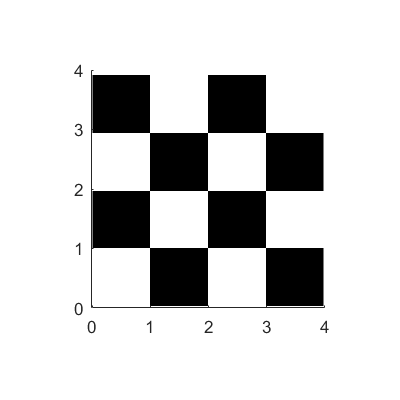
\includegraphics[width = 0.5\textwidth]{images/checkerboard.png}
        \caption{Checkerboard Pattern} \label{fig:checkerboard}
    \end{figure}
    \begin{subparts}
    % \subpart[2] What is the minimum depth of a binary decision tree that perfectly classifies the colored regions ($0 < x_1 < 4$) in Figure \ref{fig:checkerboard}, using features that only inspect either $x_1$ or $x_2$ but not both $x_1$ and $x_2$? Feel free to get creative in your use of the features $x_1$ and $x_2$ for the splits!
    
    % Since this is a binary decision tree, we can only use features that split into two branches. Some feature examples: $ceil(x_1)\%2 = 0$, \quad$2<x_1<4$, \quad$x_2<1$ or $x_2>3$

    % \begin{your_solution}[title=Your Answer,height=2cm,width=5cm]
    % \end{your_solution}
    
    
    \clearpage
    \subpart[2] What is the minimum depth of a binary decision tree that perfectly classifies the colored regions in Figure \ref{fig:checkerboard}, using \emph{only} features of the form $x_1 < c$ or of the form $x_2 < c$ for different constants $c$?
    
    \begin{your_solution}[title=Your Answer,height=2cm,width=5cm]
    \end{your_solution}

    \subpart[2] What is the minimum depth of a binary decision tree that perfectly classifies the colored regions ($0 < x_1 < 4$) in Figure \ref{fig:checkerboard}, using features that only inspect either $x_1$ or $x_2$ but not both $x_1$ and $x_2$? Feel free to get creative in your use of the features $x_1$ and $x_2$ for the splits!
    
    Since this is a binary decision tree, we can only use features that split into two branches. Some feature examples: $ceil(x_1)\%2 = 0$, \quad$2<x_1<4$, \quad$x_2<1$ or $x_2>3$

    \begin{your_solution}[title=Your Answer,height=2cm,width=5cm]
    \end{your_solution}
    
    
    \subpart[2] What is the minimum depth of a binary decision tree that perfectly classifies the colored regions in Figure \ref{fig:checkerboard}, using ANY features that involve $x_1$, $x_2$, or both? 
    
    \begin{your_solution}[title=Your Answer,height=2cm,width=5cm]
    \end{your_solution}
    
    
    
    \end{subparts}
    
    \vspace{0.5cm}
    
    \part Consider the graph below analyzing the size of tree vs. accuracy for a decision tree which has been pruned back to the vertical (red) line. Assume all of our labeled data for this task was randomly divided into a training dataset $D_{train}$, a validation data set $D_{val}$, and a test dataset $D_{test}$. The full tree was trained only on $D_{train}$, then reduced-error pruning was applied using $D_{val}$. 

    \begin{figure}[H]
      \centering
      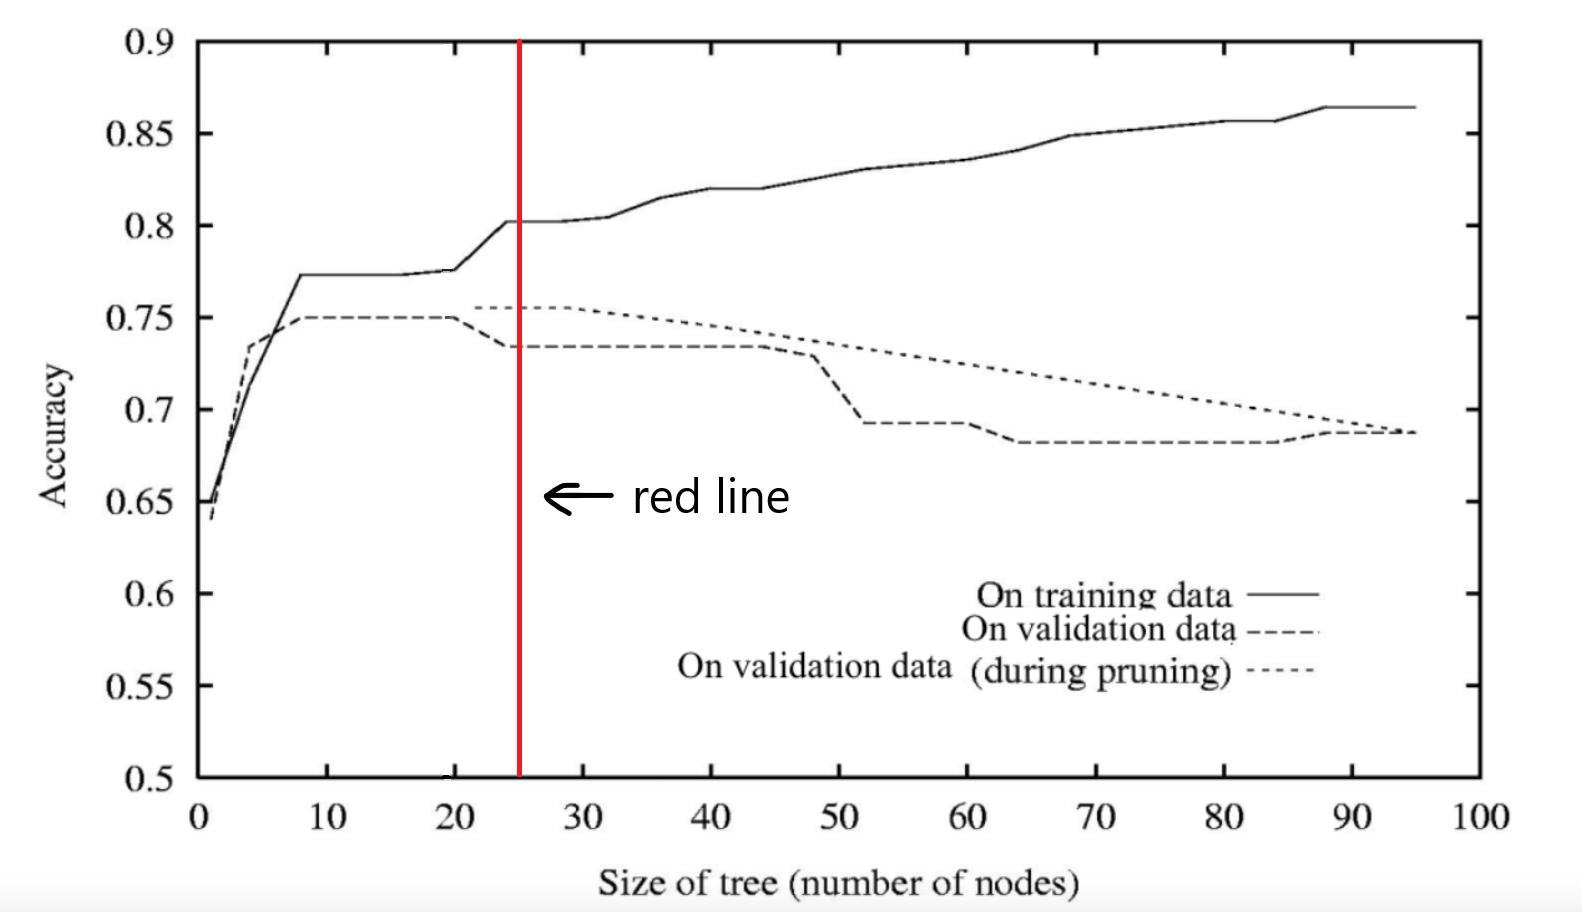
\includegraphics[width = 0.6\textwidth]{images/dtree.png}
      \caption{Pruned decision tree. The lowest running dotted curve is the validation performance of the unpruned tree as it grows during training. Finally, we prune it back to the size given by the red line with a reduced validation error (the upper running dotted curve)}
      \label{fig:dtree}
    \end{figure}
      
    \begin{subparts}
    
   \subpart[1] \sone Refer to Figure \ref{fig:dtree}. Note that $D_{test}$ was not used for training or pruning. When the size of the pruned tree is at \textbf{25 nodes}, what is its accuracy on $D_{test}$ likely to be?
    
    \begin{checkboxes}
        \choice Slightly higher than the pruned tree's accuracy on $D_{val}$
        \choice The same as the pruned tree's accuracy  on $D_{val}$
        \choice Slightly lower than the pruned tree's accuracy on $D_{val}$
    \end{checkboxes}

    
    
    \clearpage 
    
      \subpart[1] \sone Which of the following gives us the best approximation of the true error? 

    \begin{checkboxes}
        \choice Error corresponding to training data $D_{train}$
        \choice Error corresponding to validation data $D_{val}$
        \choice Error corresponding to test data $D_{test}$ 
    \end{checkboxes}
    

      \end{subparts}
    
    \part[2] \sall Which of the following are valid ways to avoid overfitting?

    {
    \checkboxchar{$\Box$} \checkedchar{$\blacksquare$}
    \begin{checkboxes}
        \choice Decrease the training set size. 
        \choice Set a threshold for a minimum number of examples required to split at an internal node. 
        \choice Prune the tree so that cross-validation error is minimal. 
        \choice Increase the tree depth.
        \choice None of the above.
    \end{checkboxes}
    }

    
    \part Consider a binary classification problem using $1$-nearest neighbors with the Euclidean distance metric. We have $N$ 1-dimensional training points $x^{(1)}, x^{(2)}, \ldots x^{(N)}$ and corresponding labels $y^{(1)}, y^{(2)}, \ldots y^{(N)}$, with $x^{(i)} \in \mathbb{R}$ and $y^{(i)} \in \{0, 1\}$. 

    Assume the points $x^{(1)}, x^{(2)}, \ldots x^{(N)}$ are in ascending order by value. If there are ties during the 1-NN algorithm, we break ties by choosing the label corresponding to the $x^{(i)}$ with lower value. 

    \textbf{NOTE:} For subparts (a) and (b), 2 models ``behave exactly the same'' when the decision boundaries produced by them are the same, leading to the same performance on all possible test data.
    
    
    \begin{subparts} 
    \subpart[2] \sone Is it possible to build a decision tree that behaves exactly the same as the 1-nearest neighbor classifier? Assume that the decision at each node takes the form of ``$x \leq t$'' or ``$x > t$'', where $t \in \mathbb{R}$.
    
    \begin{checkboxes}
        \choice Yes
        \choice No
    \end{checkboxes}
     If your answer is yes, please explain how you will construct the decision tree. If your answer is no, explain why it’s not possible. 
   
    \begin{your_solution}[title=Your answer:,height=6cm,width=15cm]
        
    \end{your_solution}
    
    \clearpage

    \subpart[3] \sall Let's add a dimension! Now the training points are 2-dimensional where $\xv^{(i)} = \left(x_1^{(i)}, x_2^{(i)}\right) \in \mathbb{R}^2$. For which of the following training sets is it possible to build a decision tree that behaves exactly the same as a 1-nearest neighbor classifier? Assume that (1) the decision at each node takes the form of ``$x_j \leq t$'' or ''$x_j > t$'', where $t \in \mathbb{R}$ and $j \in \{1,2\}$. (2) the decision tree has finite depth.
    {
    \checkboxchar{$\Box$} \checkedchar{$\blacksquare$}
    \begin{checkboxes}
        \choice Points: $\{(-5,5), (5,5)\}$, Labels: $\{0,1\}$
        \choice Points: $\{(0,-9), (0,10)\}$, Labels: $\{0,1\}$
        \choice Points: $\{(3,4), (-3,-4)\}$, Labels: $\{0,1\}$
        \choice Points: $\{(0,0), (0,1), (1,0)\}$, Labels: $\{0,0,1\}$
        \choice Points: $\{(0,0), (0,1), (1,0)\}$, Labels: $\{0,1,1\}$
        \choice Points: $\{(1,2), (3,4), (5,6)\}$, Labels: $\{0,1,1\}$
        \choice None of the above
    \end{checkboxes}
    }
    \end{subparts}
    
\newpage

\end{parts}



\clearpage
\newpage
\newpage
\sectionquestion{{\it k}-Nearest Neighbors}

\begin{parts}
    
    \begin{figure}[H]
        \centering
        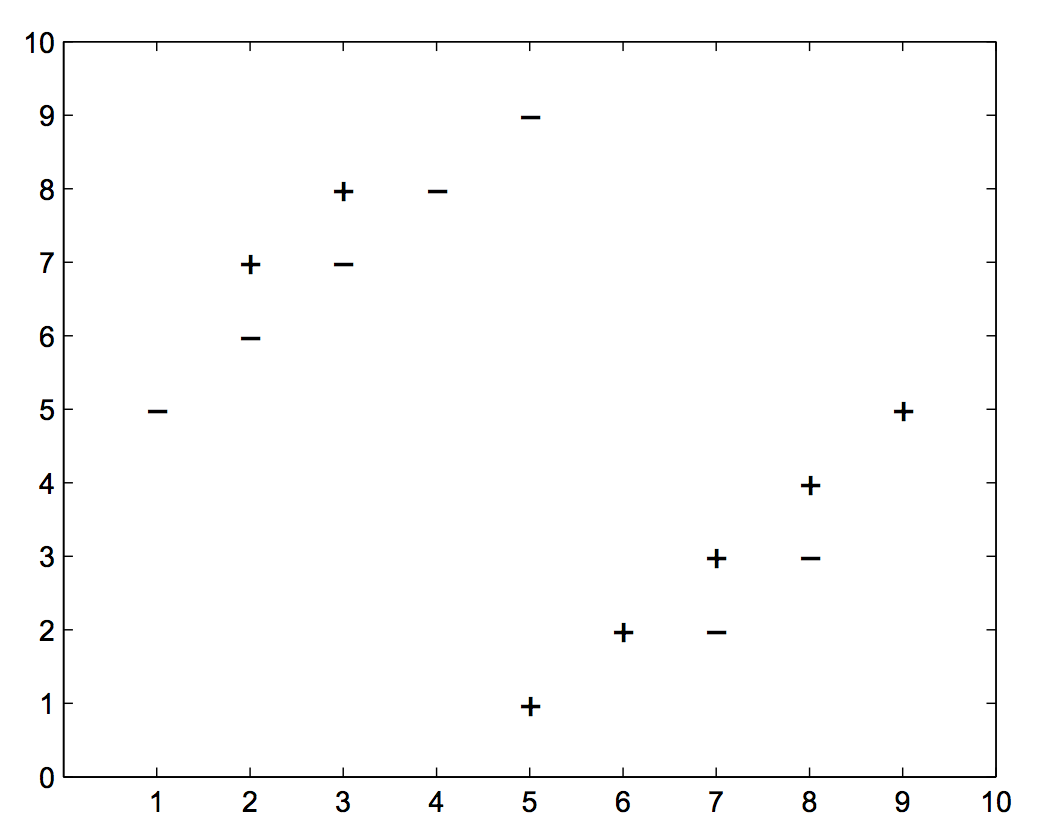
\includegraphics[width = 0.5\textwidth]{images/Q2_knn.png}
        \caption{k-NN Dataset} \label{fig:Q2_knn}
    \end{figure}

    \part Consider a $k$-nearest neighbors ($k$-NN) binary classifier which assigns the class of a test point to be the class of the majority of the $k$-nearest neighbors in the training dataset, according to the Euclidean distance metric. Assume that ties are broken by selecting one of the labels uniformly at random. 
    
    \textbf{NOTE:} An example tie scenario can occur when the classes of the 6 nearest neighbors are \{+, +, +, -, -, -\} i.e. the number of neighbors belonging to each class type is equal. In this case, you can assume the test point's class to be + or - randomly.
    
    \begin{subparts} 
    \subpart[2]Using Figure \ref{fig:Q2_knn} shown above to train the classifier and choosing $k=6$, what is the classification error on the training set? \textbf{Report your answer either as a fraction or as a decimal with 4 decimal places after the decimal point.}
    
    \begin{your_solution}[title=Your answer:,height=2cm,width=5cm]
    \end{your_solution}
    
    

    
    \clearpage 
    
    \subpart[2] \sall Let's say that we have a new test point (not present in our training data) $\xv^{\text{new}} = [3,9]^T$ that we would like to apply our $k$-NN classifier to, as seen in figure \ref{fig:Q2_knn_test}.
    
    \begin{figure}[H]
        \centering
        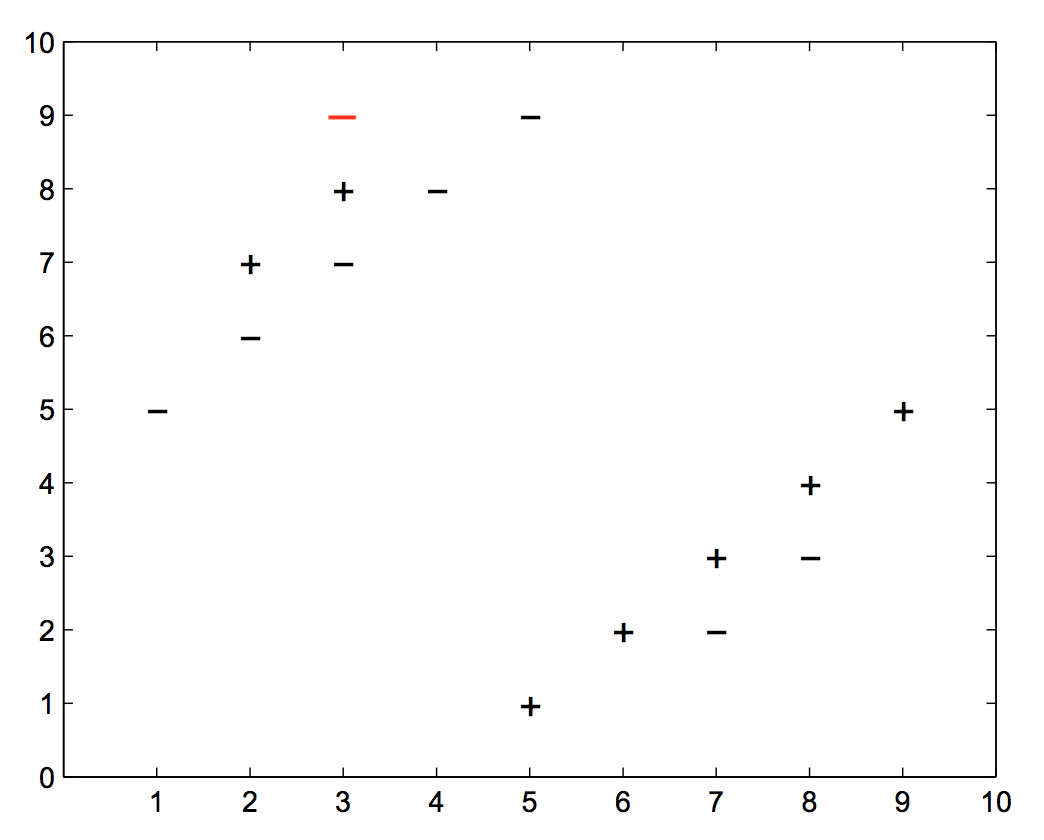
\includegraphics[width = 0.5\textwidth]{images/Q2_knn_test_point.png}
        \caption{k-NN Dataset with Test Point} \label{fig:Q2_knn_test}
    \end{figure}
    
    For which values of $k$ is this test point always correctly classified by the $k$-NN algorithm?
    
    
    {
    \checkboxchar{$\Box$} \checkedchar{$\blacksquare$}
    \begin{checkboxes}
        \choice $k$ = 1
        \choice $k$ = 5
        \choice $k$ = 9
        \choice $k$ = 12
        \choice None of the above
    \end{checkboxes}
    }
    
    
    \end{subparts}
    \part \sone Assume we have a large labeled dataset that is randomly divided into a training set and a test set, and we would like to classify points in the test set using a $k$-NN classifier. 
    
    \begin{subparts}
    
        \subpart[1] In order to minimize the classification error on this test set, we should always choose the value of $k$ which minimizes the training set error. 
    
    
    \begin{checkboxes}
        \choice True
        \choice False
    \end{checkboxes}
    
    
    \clearpage 
    \subpart[2] \sone Instead of choosing the hyperparameters by merely minimizing the training set error, we instead consider splitting the training-all data set into a training and a validation data set, and choose the hyperparameters that lead to lower validation error. Is choosing hyperparameters based on validation error better than choosing hyper-parameters based on training error?

    \begin{checkboxes}
        \choice Yes, lowering validation error instead of training error is better because lowering training error will not always help generalize our model and may lead to overfitting.
        \choice Yes, lowering validation error is better for the model because cross-validation guarantees a better test error.
        \choice No, lowering training error instead of validation error is better because lowering validation error will not help generalize our model and may lead to overfitting.
        \choice No, lowering training error is better for the model because we have to learn the training set as well as possible to guarantee the best possible test error.
    \end{checkboxes}
    


    
    \subpart[2] \sone Your friend Sally suggests that instead of splitting the original training set into separate training and validation sets, we should instead use the test set as the validation data for choosing hyperparameters. Is this a good idea? Justify your opinion with no more than 3 sentences.
    
    \begin{checkboxes}
        \choice Yes
        \choice No
    \end{checkboxes}
    

    \begin{your_solution}[title=Your answer:,height=5cm,width=15cm]
    \end{your_solution}

    \end{subparts}
    
    
    \clearpage
    
    \part[2] \sall Consider a binary $k$-NN classifier where $k=4$ and the two labels are ``triangle" and ``square".
    Consider classifying a new point $\xv =(1,1)$, where two of the $\xv$'s nearest neighbors are labeled ``triangle" and two are labeled ``square" as shown below.
    
    \begin{figure}[H]
        \centering
        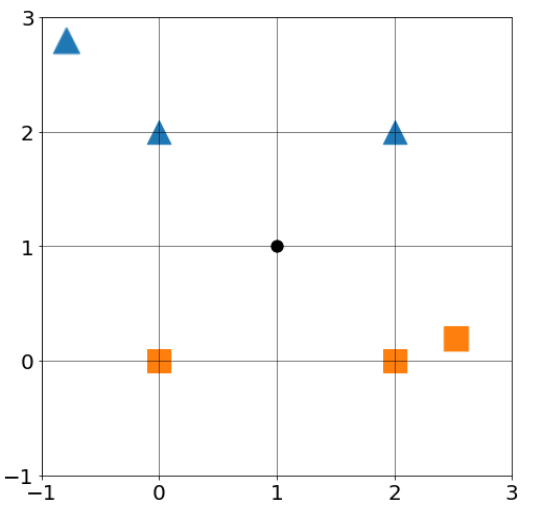
\includegraphics[width = 0.5\textwidth]{images/1-1-5.png}
        \label{Q_5knn}
    \end{figure}
    
    Which of the following methods will guarantee breaking or avoiding ties on this dataset?
    
    {%
    \checkboxchar{$\Box$} \checkedchar{$\blacksquare$}
    \begin{checkboxes}
        \choice Assign $\xv$ the label of its nearest neighbor
        \choice Flip a coin to randomly assign a label to $\xv$ (from the labels of its 4 closest points)
        \choice Use $k = 3$ instead
        \choice Use $k = 5$ instead
        \choice None of the above.
    \end{checkboxes}

    }
 

    \part[3] \sall Which of the following is/are correct statement(s) about $k$-NN models?
    {
    \checkboxchar{$\Box$} \checkedchar{$\blacksquare$}
    \begin{checkboxes}
        \choice A larger $k$ tends to give a smoother decision boundary.
        \choice To reduce the impact of noise or outliers in our data, we should increase the value $k$.
        \choice If we make $k$ too large, we could end up overfitting the data.
        \choice We can use cross-validation to help us select the value of $k$.
        \choice We should never select the $k$ that minimizes the error on the validation dataset.
        \choice None of the above.
    \end{checkboxes}
    }

    
    
    \newpage
    
    \part Consider the following data concerning the relationship between academic performance and salary after graduation. High school GPA and university GPA are two numerical features and salary is the numerical target. Note that salary is measured in thousands of dollars per year.
    
    \begin{table}[H]
        \centering
        \begin{tabular}{cccc}
            \textbf{Student ID} & \textbf{High School GPA} & \textbf{University GPA} & \textbf{Salary} \\
            1 & 2.5 & 3.8 & 45 \\
            % 2 & 3.6 & 2.4 & 55 \\
            2 & 3.3 & 3.5 & 90 \\
            3 & 4.0 & 4.0 & 142 \\
            % 5 & 2.2 & 3.2 & 88 \\
            4 & 3.0 & 2.0 & 163 \\
            5 & 3.8 & 3.0 & 2600 \\
            6 & 3.3 & 2.8 & 67 \\
            7 & 3.9 & 3.8 & unknown \\
        \end{tabular}
        \label{tab:my_label}
    \end{table}
    
    \begin{subparts}
    \subpart[2] Among Students 1 to 6, who is the nearest neighbor to Student 7, using Euclidean distance? Answer the Student ID only.
    
    \begin{your_solution}[title=Your answer:,height=2cm,width=5cm]
    \end{your_solution}
    
    
    
    \subpart[2] Now, our task is to predict the salary Student 7 earns after graduation. We apply $k$-NN to this regression problem: the prediction for the numerical target (salary in this example) is equal to the average of salaries for the top $k$ nearest neighbors. If $k=3$, what is our prediction for Student 7's salary? Be sure to use the same unit of measure (thousands of dollars per year) as the table above. \\
    \textbf{Round your answer to the nearest integer.}
    
    \begin{your_solution}[title=Your answer:,height=2cm,width=5cm]
    \end{your_solution}
    
    

    \subpart[2] \sall Suppose that the first 6 students shown above are only a subset of your full training data set, which consists of 10,000 students. We apply $k$-NN regression using Euclidean distance to this problem and we define training loss on this full data set to be the mean squared error (MSE) of salary. Now consider the possible consequences of modifying the data in various ways. Which of the following changes \textbf{could} have an effect on training loss on the full data set as measured by mean squared error (MSE) of salary?
    
    
        
    
    {
    \checkboxchar{$\Box$} \checkedchar{$\blacksquare$}
    \begin{checkboxes}
        \choice Rescaling only ``High School GPA" to be a percentage of 4.0
        \choice Rescaling only ``University GPA" to be a percentage of 4.0
        \choice Rescaling both High School GPA and University GPA by the same percentage/scale
        \choice None of the above.
    \end{checkboxes}
    }

    
    
    \end{subparts}

    \clearpage
    
    \begin{EnvFullwidth}
    \part An archaeologist discovers a 242 kilobyte 8-inch floppy disk buried beneath the hedges near Wean Hall. The floppy disk contains a few hundred black and white images of 3x3 pixels. You are asked to classify them as either a photo ($y=+$) or artwork ($y=-$) to aid in the analysis. 
    
    You build a k-Nearest Neighbor (k-NN) classifier trained on a training dataset obtained from the web (converted to similarly small black and white images). Suppose you are informed that each image is represented as a $3 \times 3$ matrix $\xv$ of binary values and you plan to use Hamming distance to measure the distance between each pair of $3 \times 3$ pixel images as follows: 
    $$d(\uv, \mathbf{v}) = \sum_{i=1}^3 \sum_{j=1}^3 \mathbbm{1}(\uv_{i,j} \neq \vv_{i,j}) = \text{the number of pixels that differ between } \uv \text{ and } \vv$$
    While calculating the distance metric, if there is a tie in distance among the points competing for $k$ nearest points, the classifier increases $k$ to include all those tied points in the majority vote. If, in the end, there is a tie in the vote, your classifier returns $\hat{y}=?$. 
    You can try out your k-NN implementation on the images below.
    
    \begin{table}[H]
        \begin{center}
        \begin{tabular}{ccccccccccc}
            \toprule
             i & $y$ & $x_{1,1}$ & $x_{1,2}$ & $x_{1,3}$ & $x_{2,1}$ & $x_{2,2}$ & $x_{2,3}$ & $x_{3,1}$ & $x_{3,2}$ & $x_{3,3}$  \\
             \midrule
             1 & $+$ & 0 & 0 & 1 & 0 & 1 & 1 & 0 & 0 & 0 \\
             2 & $+$ & 1 & 0 & 1 & 0 & 1 & 0 & 1 & 0 & 0 \\
             3 & $+$ & 0 & 1 & 0 & 1 & 1 & 1 & 1 & 0 & 1 \\
             4 & $-$ & 0 & 0 & 1 & 0 & 0 & 0 & 0 & 0 & 0 \\
             5 & $-$ & 1 & 0 & 1 & 1 & 1 & 0 & 0 & 1 & 1 \\
             \bottomrule
        \end{tabular}
        \end{center}
     \caption{Training Data}
     \label{tab:knnimages}
    \end{table}
    
    % Below are the test points on which you evaluate the classifier. Above we include the distance of each of these test points to each of the training points.
    
    \begin{table}[H]
        \begin{center}
        \begin{tabular}{cccccccccc}
            \toprule
             i & $x_{1,1}$ & $x_{1,2}$ & $x_{1,3}$ & $x_{2,1}$ & $x_{2,2}$ & $x_{2,3}$ & $x_{3,1}$ & $x_{3,2}$ & $x_{3,3}$  \\
             \midrule
             6 & 1 & 0 & 1 & 0 & 0 & 0 & 1 & 0 & 1 \\
             7 & 0 & 0 & 1 & 0 & 0 & 1 & 1 & 1 & 0 \\
             \bottomrule
        \end{tabular}
        \end{center}
     \caption{Test Data}
     \label{tab:knnimages}
    \end{table}
    
    \end{EnvFullwidth}
    
    \clearpage
    
    \begin{subparts}
    
    \subpart[1] What is the distance between $\xv^{(2)}$ and $\xv^{(6)}$? \\
        \begin{your_solution}[title=Your answer:,height=2cm,width=5cm]
        \end{your_solution}
        
    % \subpart[1] \textbf{Select one:} What would a k-NN classifier with $k=1$ predict as the label for test point $\xv^{(7)}$?
    %     \begin{checkboxes}
    %      \choice $\hat{y}=+$
    %      \choice $\hat{y}=-$
    %      \choice $\hat{y}=?$
    %     \end{checkboxes}
        
    \subpart[1] \textbf{Select one:} What would a k-NN classifier with $k=3$ predict as the label for test point $\xv^{(7)}$?
        \begin{checkboxes}
         \choice $\hat{y}=+$
         \choice $\hat{y}=-$
         \choice $\hat{y}=?$
        \end{checkboxes}
        
    \subpart[1] \textbf{Select one:} What would a k-NN classifier with $k=5$ predict as the label for test point $\xv^{(7)}$?
        \begin{checkboxes}
         \choice $\hat{y}=+$
         \choice $\hat{y}=-$
         \choice $\hat{y}=?$
        \end{checkboxes}
    
    \subpart[2] \textbf{Short answer:} Your friend says that you should try using Euclidean distance because it might give better results. Do you agree that switching could lead to lower test error? Why or why not? \\
        \begin{your_solution}[title=Your answer:, height=5cm]
            % YOUR ANSWER
            % TODO: write the answer
        \end{your_solution}
        
    \end{subparts}
    \clearpage
    \part Let's say you have a large labeled dataset and you want to train a $k$-NN classifier on it. You have decided you're going to perform hyperparameter optimization by performing a grid search. The specific hyperparameters you choose to vary are the value of $k$ and the distance metric. You also decide you want to perform cross-validation when assessing these different classifiers during the course of your grid search.
    \begin{subparts}
    \subpart[2] Let's say there are 5 different values of $k$ you wish to test (3, 5, 7, 9, 11), 2 different distance metrics (Euclidean distance and Hamming distance) and you choose to do 10-fold cross-validation. How many different classifiers will you end up training in total?
        
        \begin{your_solution}[title=Your answer:,height=2cm,width=5cm]
        \end{your_solution}
        
    \subpart[1] \sone What is the trade-off between using cross-validation error in this example as opposed to simply calculating the validation error on a single held-out validation set?

        \begin{checkboxes}
            \choice Cross-validation error has a lower variance, but is less computationally expensive to calculate.
            \choice Cross-validation error has a lower variance, but is more computationally expensive to calculate.
            \choice Cross-validation error has a higher variance, but is less computationally expensive to calculate.
            \choice Cross-validation error has a higher variance, but is more computationally expensive to calculate.
        \end{checkboxes}
    

    \end{subparts}
\end{parts}
\clearpage
\newpage
\sectionquestion{Perceptron}
\begin{parts}
    \part[1] \sone Consider running the online perceptron algorithm on some sequence of examples $S$ (an example is a data point and its label). Let $S^\prime$ be the same set of examples as $S$, but presented in a different order.
    
    \emph{True or False:} The online perceptron algorithm is guaranteed to make the same number of mistakes on $S$ as it does on $S^\prime$.

    \begin{checkboxes}
        \choice True
        \choice False
    \end{checkboxes}


    
    \part[3] \sall Suppose we have a perceptron whose inputs are 2-dimensional vectors and each feature vector component is either 0 or 1, i.e., $x_i \in \{0,1\}$. The prediction function is $y = \operatorname{sign}(w_1x_1 + w_2x_2 + b)$, and
    $$
    \operatorname{sign}(z) = 
    \begin{cases}
    1, & \textrm{ if } z > 0\\
    0, & \textrm{ otherwise}.
    \end{cases}
    $$
    Which of the following functions can be implemented with the above perceptron? That is, for which of the following functions does there exist a set of parameters $w,b$ that correctly define the function. 

    {
    \checkboxchar{$\Box$} \checkedchar{$\blacksquare$}
    \begin{checkboxes}
        \choice AND function, i.e., the function that evaluates to 1 if and only if all inputs are 1, and 0 otherwise.
        \choice OR function, i.e., the function that evaluates to 1 if and only if at least one of the inputs are 1, and 0 otherwise.
        \choice XOR function, i.e., the function that evaluates to 1 if and only if the inputs are not all the same. For example
        $$
        \operatorname{XOR}(1,0) = 1, \textrm{ but } \operatorname{XOR}(1,1) = 0.
        $$
        % $$
        % \operatorname{XOR}(1,-1) = 1, \textrm{ but } \operatorname{XOR}(1,1) = -1.
        % $$
        \choice None of the above.
    \end{checkboxes}
    }

    
    
    
    \part[2]\sone Suppose we have a dataset $\left\{ \left(\xv^{(1)},y^{(1)}\right),\ldots, \left(\xv^{(N)},y^{(N)}\right) \right\}$, where $\xv^{(i)} \in \mathbb{R}^M$, $y^{(i)}\in\{+1,-1\}$. We would like to apply the perceptron algorithm on this dataset. Assume there is no intercept term. How many parameter values is the perceptron algorithm learning?

    \begin{checkboxes}
        \choice $N$
        \choice $N\times M$
        \choice $M$
    \end{checkboxes}


    
    \clearpage
    
    \part[2] \sone The following table shows a data set and the number of times each point is misclassified during a run of the perceptron algorithm. What is the separating plane $\boldsymbol\theta$ found by the algorithm, i.e. $\boldsymbol\theta = [b, \theta_1, \theta_2, \theta_3]$? Assume that the initial weights are all zero.
 
    \begin{center}
    \begin{tabular}{||c c c c c||}
        \hline
         $x_1$ & $x_2$ & $x_3$ & $y$ & \text{Times Misclassified} \\ \hline
        2 & 1 & 5 & 1 & 10 \\
        \hline
        5 & 3 & 3 & 1 & 5 \\
        \hline
        1 & 6 & 2 & 1 & 8 \\
        \hline
        7 & 2 & 1 & -1 & 2 \\
        \hline
        3 & 2 & 6 & -1 & 3 \\
        \hline
    \end{tabular}
    \end{center}
    
    \begin{checkboxes}
        \choice $[18,25,14,34]$ 
        \choice $[18,30,63,61]$ 
        \choice $[16,56,18,47]$ 
        \choice $[18,52,19,47]$ 
    \end{checkboxes}
    
    
    
    

    
    \part[2] \sall Which of the following is/are correct statement(s) about the mistake bound of the perceptron algorithm?

    {%
    \checkboxchar{$\Box$} \checkedchar{$\blacksquare$}
    \begin{checkboxes}
        \choice If the minimum distance from any data point to the separating hyperplane is increased, without any other change to the data points, the mistake bound will also increase.
        \choice If the whole dataset is shifted away from origin, then the mistake bound will also increase.
        \choice If the pair-wise distance between data points is increased, i.e. the data is scaled by some constant value, then the mistake bound will also increase.
        \choice The mistake bound is linearly inverse-proportional to the minimum distance of any data point to the separating hyperplane of the data.
        \choice None of the above.
    \end{checkboxes}
    }


    
    \part[2] \sone Suppose we have data whose examples are of the form $[x_1,x_2]$, where $x_1 - x_2 = 0$. We do not know the label for each element. Suppose the perceptron algorithm starts with $\bm{\theta} = [3,5]$; which of the following values will $\bm{\theta}$ never take on in the process of running the perceptron algorithm on the data?

    \begin{checkboxes}
        \choice $[-1,1]$
        \choice $[4,6]$
        \choice $[-3,0]$
        \choice $[-6,-4]$
    \end{checkboxes}

    
    \clearpage 
    
    \part[2] \sall Consider the linear decision boundary below and the test dataset shown. Which of the following weight vectors $\bm{\theta}$ is paired with its corresponding test error on this dataset? (Note: Assume the decision boundary is fixed and does not change while evaluating error.)

    {%
    \checkboxchar{$\Box$} \checkedchar{$\blacksquare$}
    \begin{checkboxes}
        % \choice $\bm{\theta} = [2,1]$, error  = 5/13
        \choice $\bm{\theta} = [-2,1]$, error = 5/13
        \choice $\bm{\theta} = [2,-1]$, error = 8/13
        \choice $\bm{\theta} = [2,-1]$, error = 5/13
        \choice $\bm{\theta} = [-2,1]$, error = 8/13
        % \choice $\bm{\theta} = [-2,-1]$, error = 8/13
        \choice None of the above.
    \end{checkboxes}
    }
    
    
    \begin{figure}[H]
        \centering
        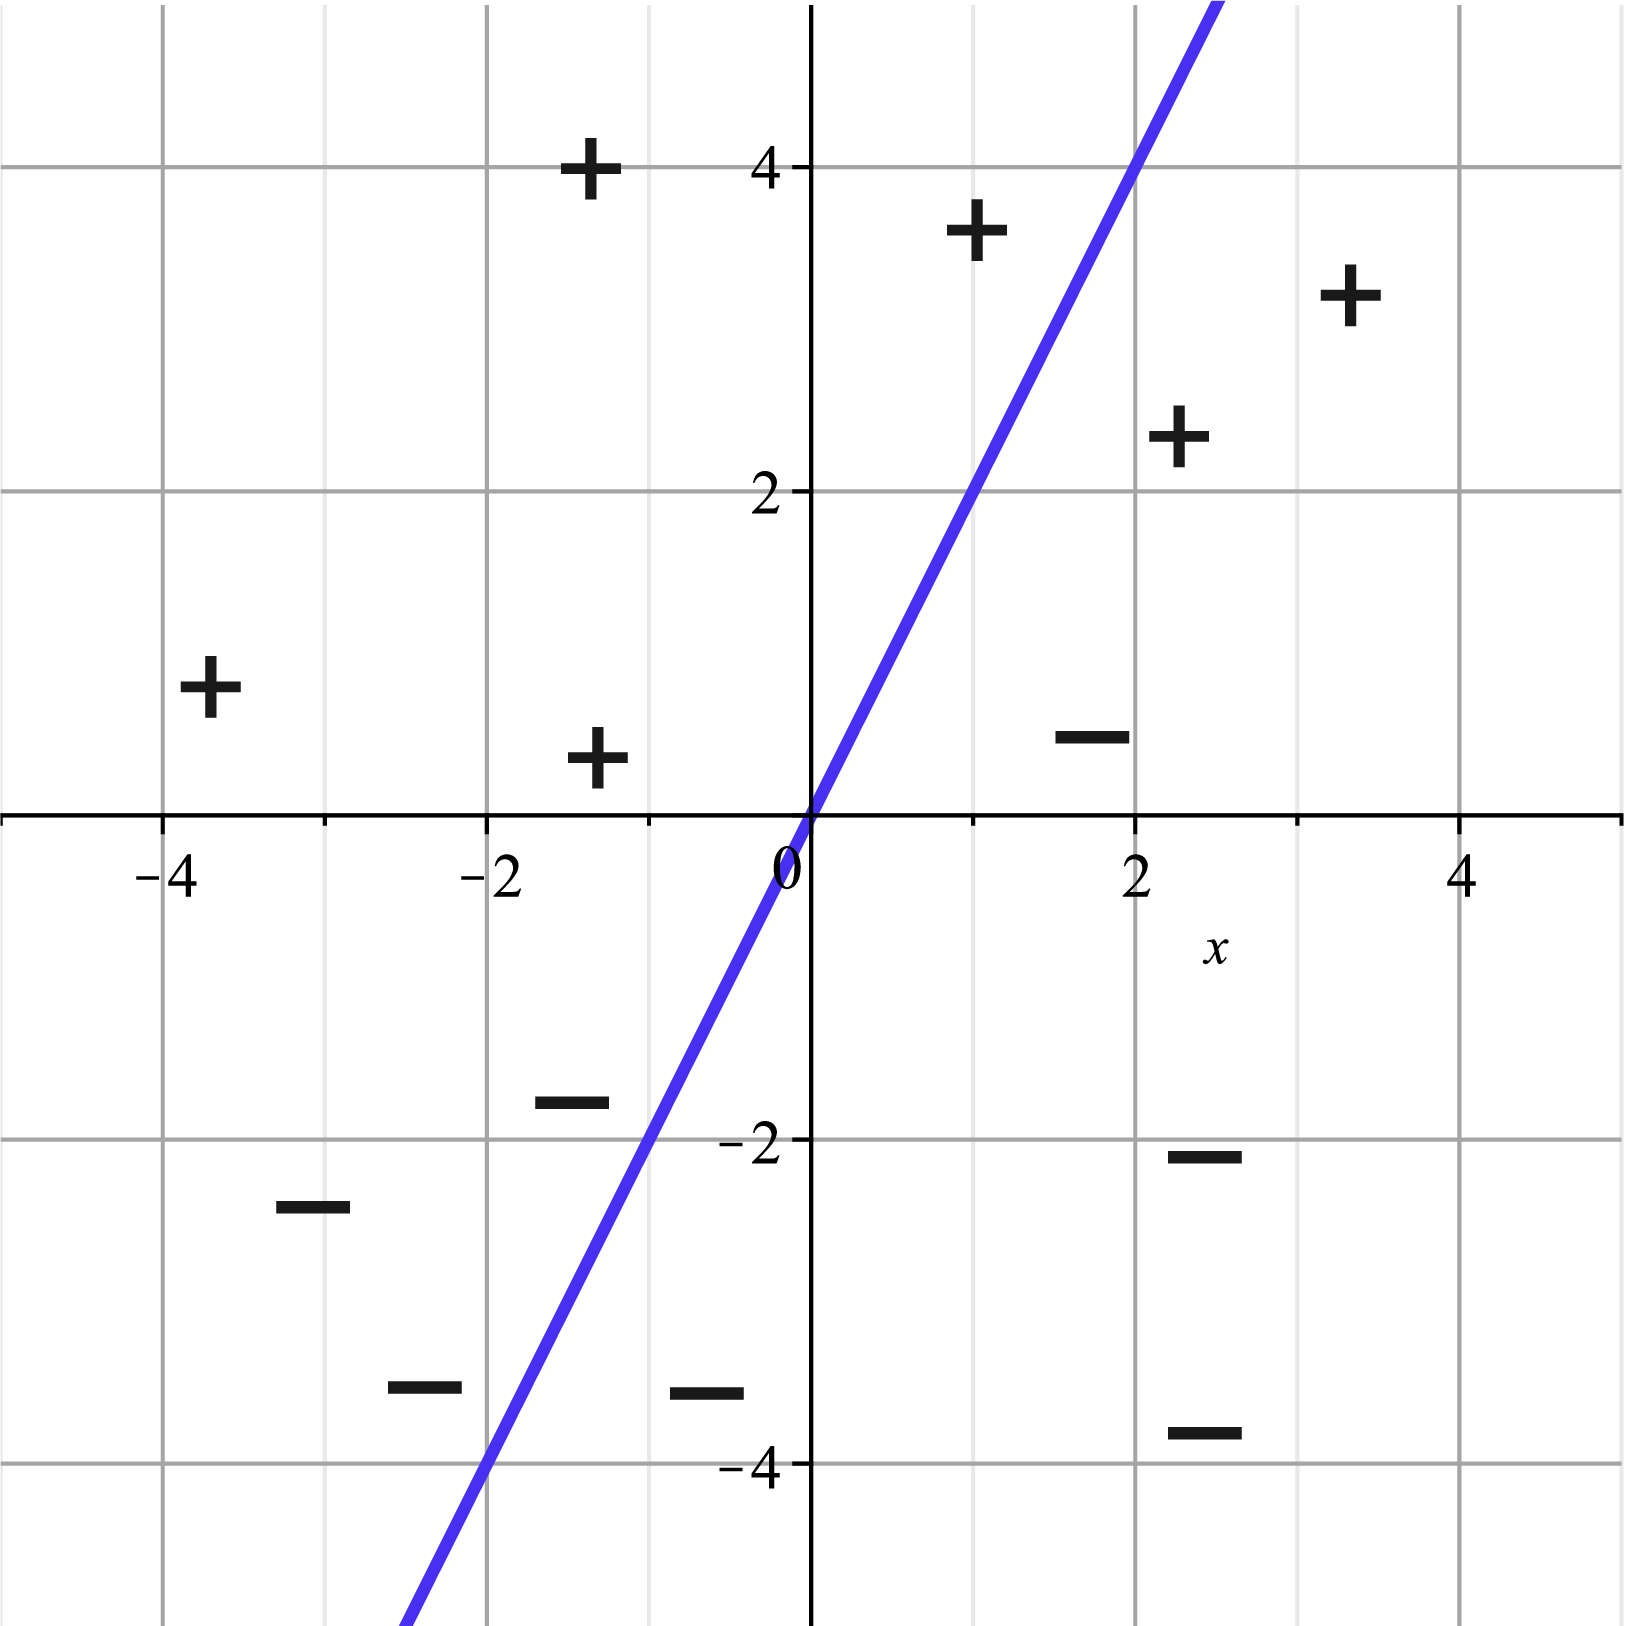
\includegraphics[width = 0.5\textwidth]{images/perceptron_boundary.png}
        \label{Q_10perceptron}
    \end{figure}
    
    
    \clearpage
    
    
    \part The following problem will walk you through an application of the Perceptron Mistake Bound. The following table shows a linearly separable dataset, and your task will be to determine the mistake bound for the dataset.

    \textbf{NOTE:} The proof of the perceptron mistake bound requires that the optimal linear separator passes through the origin. To make the linear separator pass through the origin, we fold the bias into the weights and prepend a 1 to each training example's input. The original data is on the left, and the result of this prepending is shown on the right. \textbf{Be sure to use the modified dataset on the right in your calculations.}
    
    \begin{center}
    \begin{tabular}{||c c c||}
        \hline
         $x_1$ & $x_2$ & $y$ \\ [0.5ex]
        \hline\hline
        -2 & 2 & 1 \\
        \hline
        -1 & -3 & -1 \\
        \hline
        -2 & -3 & -1 \\
        \hline
        0 & 1 & 1 \\
        \hline
        2 & -1 & 1 \\
        \hline
    \end{tabular}
    \hspace{4em}
    \begin{tabular}{||c c c c||}
        \hline
        $\bm{x_0}$ & $x_1$ & $x_2$ & $y$ \\ [0.5ex]
        \hline\hline
        \textbf{1} & -2 & 2 & 1 \\
        \hline
        \textbf{1} & -1 & -3 & -1 \\
        \hline
        \textbf{1} & -2 & -3 & -1 \\
        \hline
        \textbf{1} & 0 & 1 & 1 \\
        \hline
        \textbf{1} & 2 & -1 & 1 \\
        \hline
    \end{tabular}
    \end{center}
    
    \begin{subparts}
        \subpart[2] Compute the radius $R$ of the ``circle" centered at the origin that bounds the data points. \\
        \textbf{Round to 4 decimal places after the decimal point.}
        
        \begin{your_solution}[title=Radius:,height=2cm,width=5cm]
        \end{your_solution}
        
        
        
        \subpart[2] Assume that the linear separator with the largest margin is given by \[\thetav^{*T}\begin{bmatrix}
        1 \\
        x_1 \\
        x_2 
        \end{bmatrix} = 0, \text{, where } \thetav^* = \begin{bmatrix}
        6 \\
        3 \\
        4 
        \end{bmatrix}
        \]
        Now, compute the margin of the dataset.\\
        \textbf{Round to 4 decimal places after the decimal point.}
        
        \begin{your_solution}[title=Margin:,height=2cm,width=5cm]
        \end{your_solution}
        
        
        
        \subpart[1] Based on the above rounded values, what is the theoretical perceptron mistake bound for this dataset, given this linear separator? \\ \textbf{Round to 4 decimal places after the decimal point.}
        
        \begin{your_solution}[title=Mistake Bound:,height=2cm,width=5cm]
        \end{your_solution}
        
        
        
        % \clearpage
        
        
    \end{subparts}
    \clearpage
\end{parts}
\clearpage
\newpage
\sectionquestion{Linear Regression}
\begin{parts}
    
    \part \label{Q7_linear_regression} Consider the following dataset:
    \begin{table}[H]
    \centering
        \begin{tabular}{llllll}
        x & 9.0 & 2.0 & 6.0 & 1.0 & 8.0 \\
        y & 1.0 & 0.0 & 3.0 & 0.0 & 1.0
        \end{tabular}
    \end{table}
    Let $\bm{x}$ be the vector of datapoints and $\bm{y}$ be the label vector. Here, we are fitting the data using gradient descent, and our objective function is $J(w, b) = \dfrac{1}{N}\sum\limits_{i=1}^N (wx_i + b - y_i)^2$ where $N$ is the number of data points, $w$ is the weight, and $b$ is the intercept.

    % TODO: format
    \textbf{Note:} Showing your work in these questions is optional, but it is recommended to help us understand where any misconceptions may occur. We may give partial credit for correct work if your answer is incorrect.
    
    \begin{subparts}

         \subpart[2]  If we initialize the weight as $3.0$ and intercept as $0.0$, what is the gradient of the loss function with respect to the weight $w$, calculated over all the data points, in the first step of the gradient descent update? 
        % Round to 2 decimal places after the decimal point.
        \\ \textbf{Round to 4 decimal places after the decimal point.}
        
        \begin{your_solution}[title=Gradient:,height=2cm,width=6cm]
        \end{your_solution}

        \begin{your_solution}[title=Work,height=6cm]
        % YOUR ANSWER
        % TODO: write the answer
        \end{your_solution}
    \clearpage


    \subpart[2] What is the gradient of the loss function with respect to the intercept $b$, calculated over all the data points, in the first step of the gradient descent update?

        \begin{your_solution}[title=Gradient:,height=2cm,width=6cm]
        \end{your_solution}

        \begin{your_solution}[title=Work,height=8cm]
        % YOUR ANSWER
        \end{your_solution}


    
    
    
    \subpart[2]  Let the learning rate be $0.01$. Perform one step of gradient descent on the data. Fill in the following blanks with the value of the weight and the value of the intercept after this step. 
        % Round to 2 decimal places after the decimal point.
        \\ \textbf{Round to 4 decimal places after the decimal point.}
    
    \begin{your_solution}[title=Weight:,height=2cm,width=6cm]
    \end{your_solution}
    
    
    \begin{your_solution}[title=Intercept:,height=2cm,width=6cm]
    \end{your_solution}

    
    

    
    \end{subparts}

    \clearpage
    
    \part Consider a dataset $\Dc_1 = \{(x^{(1)}, y^{(1)}), \ldots, (x^{(N)}, y^{(N)})\}$. Assume the linear regression model that minimizes the mean-squared error on $\Dc_1$ is $y = w_1 x + b_1$. 
    
    \begin{subparts}
        \subpart[2] \sone Now, suppose we have the dataset
        $\Dc_2 = \{(x^{(1)} + \alpha,\, y^{(1)} + \beta), \ldots, (x^{(N)} + \alpha,\, y^{(N)} + \beta)\}$ where $\alpha > 0, \beta > 0$ and $w_1 \alpha \neq \beta$. Assume the linear regression model that minimizes the mean-squared error on $\Dc_2$ is $y = w_2 x + b_2$. Select the correct statement about $w_1, w_2, b_1, b_2$ below. Note that the statement should hold no matter what values $\alpha, \beta$ take on within the specified constraints.

        \begin{checkboxes}
            \choice $w_1 = w_2, b_1 = b_2$
            \choice $w_1 \neq w_2, b_1 = b_2$
            \choice $w_1 = w_2, b_1 \neq b_2$
            \choice $w_1 \neq w_2, b_1 \neq b_2$
        \end{checkboxes}
        
    
        
        
        \subpart[2]  We decide to ask a friend to analyze $\Dc_1$; however, he makes a mistake by duplicating a subset of the rows in $\Dc_1$.  Explain why the linear regression parameters that minimize mean-squared error on the duplicated data \textit{may} differ from the parameters learned on $\Dc_1$, i.e. $w_1$ and $b_1$.
        
        \begin{your_solution}[title=Your answer:,height=4cm,width=15cm]
        \end{your_solution}
        
        
    \end{subparts}
    
    \part We wish to learn a linear regression model on the dataset $\Dc = \{(\bm{x}^{(1)}, y^{(1)}), \ldots, (\bm{x}^{(N)}, y^{(N)})\}$ where $\bm{x} \in \mathbb{R}^k$. For this question, define the \emph{log-cosh loss} as
\[
    \ell(\hat y, y) = \log(\cosh(\hat y - y)) 
\]
In this question, $\log$ function has base $\textbf{e}$.

In particular, for a given point $\bm{x}^{(i)}$, the log-cosh loss of a model with parameters $\bm\theta$ is 
\[
     J^{(i)}(\bm\theta) = \log\left(\cosh\left(\bm\theta^T\bm{x}^{(i)} - y^{(i)}\right)\right) 
\] We are interested in minimizing loss over our training data, so we minimize the average log-cosh loss over all points in $\Dc$. 
    \newpage
    \begin{subparts}
        % \subpart[2]  
        % What is the objective $J(\bm\theta)$ in this setting? 
        
        % \begin{your_solution}[title=Your answer:,height=4cm,width=15cm]
        % \end{your_solution}

        
        \subpart[3] 
         What is the partial derivative of $J^{(i)}(\bm\theta)$ with respect to the $j^{\textrm{th}}$ parameter, $\theta_j$? It may be helpful to know that $\frac{d}{dx}\cosh(x) = \sinh(x)$. 
         
        \begin{your_solution}[title=Your answer:,height=6cm,width=15cm]
        \end{your_solution}
        
        \subpart[2] 
         What is the gradient of $J^{(i)}(\bm\theta)$ with respect to the entire parameter vector $\bm\theta$?
         
        \begin{your_solution}[title=Your answer:,height=4cm,width=15cm]
        \end{your_solution}
        
        % \subpart[2] To find the optimal parameter vector $\bm\theta^*$ that minimizes $J(\bm\theta)$, we again decide to use gradient descent. Write pseudocode that performs gradient descent for one iteration. Set learning rate $\alpha = 0.1$ and initialize $\bm\theta$ to be the zero vector. You may use $\texttt{gradient[i]}$ as a variable that contains your answer to part (c) in your pseudocode. Limit your answer to 10 lines.

        \subpart[2] Let 
        
        \begin{center} $J(\bm\theta) = \frac1N \sum\limits_{i=1}^{N} J^{(i)}(\bm\theta).$ 
        \end{center}
        
        To find the optimal parameter vector $\bm\theta^*$ that minimizes $J(\bm\theta)$, we again decide to use gradient descent. Write pseudocode that performs gradient descent for one iteration. Set the learning rate to $\alpha = 0.1$ and initialize $\bm\theta$ to be the zero vector. You may use $\texttt{gradient[i]}$ as a variable that contains your answer to part (b) in your pseudocode. Limit your answer to 10 lines.

        \begin{your_solution}[title=Your Answer,height=5.5cm,width=15cm]
            
        % INSERT YOUR ANSWER BELOW
        \begin{your_code_solution}

        \end{your_code_solution}
            
        \end{your_solution}
        
        
    \end{subparts}
    
\end{parts}



\end{questions}

\newpage
\section{Collaboration Questions}
After you have completed all other components of this assignment, report your answers to these questions regarding the collaboration policy. Details of the policy can be found \href{http://www.cs.cmu.edu/~mgormley/courses/10601/syllabus.html}{here}.
\begin{enumerate}
    \item Did you receive any help whatsoever from anyone in solving this assignment? If so, include full details.
    \item Did you give any help whatsoever to anyone in solving this assignment? If so, include full details.
    \item Did you find or come across code that implements any part of this assignment? If so, include full details.
\end{enumerate}

\begin{your_solution}[height=6cm]
% YOUR ANSWER 

\end{your_solution}
    

\end{document}